\documentclass[11pt]{article}
\usepackage[a4paper,margin=1in]{geometry}
\usepackage{amsmath,amssymb,amsfonts,mathtools}
\usepackage{booktabs,array}
\usepackage{graphicx}
\usepackage{hyperref}
\usepackage{enumitem}
\usepackage[title]{appendix}
\usepackage{microtype}
\setlist{nosep}
\numberwithin{equation}{section}

\newcommand{\E}{\mathbb{E}}
\newcommand{\Var}{\operatorname{Var}}
\newcommand{\Cov}{\operatorname{Cov}}
\newcommand{\MSNR}{\operatorname{MSNR}}

\hypersetup{
  pdftitle={Unified Boundary Field Theory of Interest Rates III: The Stochastic Long Boundary},
  pdfauthor={Sachin Oza},
  pdfsubject={A one-Brownian equilibrium term-structure field with a stochastic realised long boundary},
  pdfkeywords={
    term structure of interest rates,
    stochastic long boundary,
    Robin boundary condition,
    instantaneous rolling forward rates,
    Kolmogorov forward equation,
    market signal-to-noise ratio,
    boundary field theory
  },
  colorlinks=true,
  linkcolor=blue,
  citecolor=blue,
  urlcolor=blue
}

\title{\textbf{Unified Boundary Field Theory of Interest Rates III: The Stochastic Long Boundary}\\[0.5em]
\large A One-Brownian Equilibrium Field with a Stochastic Realised Long Boundary}
\author{Sachin Oza}
\date{August 2026}

\begin{document}
\maketitle

\begin{abstract}
Earlier papers in the Unified Boundary Field Theory (UBFT) represented deviations from the long-run interest rate by maturity modes that decay toward a fixed asymptotic level $x_\infty$ \cite{OzaIRFR,OzaShortBoundary}. The restriction appeared benign, not least because it is consistent with the widespread use of one-factor equilibrium term-structure models built around a fixed long-run anchor. Within the UBFT framework, however, the distinction between the equilibrium long-maturity level and the realised long-maturity state is material since the axioms identify $x_\infty$ as an equilibrium anchor, but do not require the realised infinite-maturity rate to equal $x_\infty$ pathwise. Imposing that property through the cross-sectional ansatz is therefore an additional closure restriction and may be stronger than the rolling-coordinate invariance required by Axiom 2.

This paper removes that restriction by introducing the realised long-boundary state $X_t:=\lim_{\tau\to\infty}x_t^R(\tau)$ directly into the repeated-root Robin representation. The resulting field preserves the short-boundary geometry of Paper II \cite{OzaShortBoundary} while separating the realised long-boundary $X_t$ from its equilibrium anchor $x_\infty$. The enlarged curve is then subjected to the same affine Kolmogorov-forward, equilibrium-transport and rolling-consistency conditions, consistent with the theory. The resulting coefficient-matching theorem shows that, when the short and long boundary innovations share one Brownian direction, the projected maturity diffusion equals the original Axiom-2 drift--diffusion kernel at every maturity. Importantly, the deterministic compatibility condition required by this identity is exactly the Robin identification already obtained in Paper II \cite{OzaShortBoundary}, rather than a new restriction.

The construction therefore extends UBFT from a fixed realised long boundary to a stochastic long-boundary field without increasing Brownian dimension. Under the strict Axiom-2 closure, the two economically distinct boundary coordinates are driven by one dynamically independent stochastic state: after an affine shift, the short and long boundaries are pathwise proportional. A broader imperfect-correlation model remains available as an extension, but it is not required merely because $X_t$ is stochastic.
\end{abstract}

\section{Introduction: an implicit restriction in the earlier ansatz}

The Unified Boundary Field Theory (UBFT) treats the term structure of instantaneous rolling forward rates (IRFRs) as a maturity field constrained by the Kolmogorov forward equation (KFE), rolling-coordinate consistency, equilibrium moment transport and admissible boundary behaviour. Paper I develops the affine one-Brownian construction and its common maturity kernel \cite{OzaIRFR}. Paper II classifies the free/Neumann and fixed/Dirichlet short-boundary limits and derives the mixed/Robin condition as the most economically relevant boundary regime \cite{OzaShortBoundary}.

The Paper II Robin representation is
\begin{equation}
 x_t^R(\tau)=x_\infty+[A_{R,t}+B_{R,t}\tau]e^{-a^2\tau},
 \qquad \tau=T-t.
\end{equation}
It follows immediately that
\begin{equation}
 \lim_{\tau\to\infty}x_t^R(\tau)=x_\infty
\end{equation}
for every realised path. That conclusion is mathematically correct, but it follows from the chosen cross-sectional ansatz rather than from a separate pathwise requirement of the axioms.

The relevant distinction is between the equilibrium long boundary
\begin{equation}
 X_e:=\lim_{\tau\to\infty}x_e^R(\tau)=x_\infty
\end{equation}
and the realised long-boundary state
\begin{equation}
 X_t:=\lim_{\tau\to\infty}x_t^R(\tau).
\end{equation}
The earlier representation imposed $X_t\equiv x_\infty$ by construction. This was easy to overlook because a fixed long-run anchor is familiar from one-factor equilibrium term-structure models and a representation of the form ``constant plus decaying modes'' appears natural. Within UBFT, however, Axiom 2 requires rolling-coordinate consistency but does not visibly require the realised long boundary to be deterministic while the remainder of the field is stochastic. The infinite-maturity boundary is an asymptotic state of the fitted field rather than the rate on a literally infinite-maturity traded instrument.

The purpose of this paper is therefore narrow: to relax only the pathwise identification $X_t\equiv x_\infty$ while preserving the repeated-root Robin maturity family, the equilibrium anchor $x_\infty$, the affine KFE structure and the common Axiom-2 drift--diffusion kernel. The resulting model nests Paper II because
\begin{equation}
 X_t=x_\infty
 \quad\Longrightarrow\quad
 \text{the Paper II Robin field}.
 \label{eq:paper2nestingintro}
\end{equation}

The argument proceeds in four steps. First, the fixed long boundary is relaxed within the existing repeated-root maturity family. Second, the Robin condition determines the repeated-root coefficient from the short and long boundary states. Third, the projected field diffusion is matched to the Axiom-2 common kernel under a single Brownian innovation. Fourth, the compatibility condition required by that match is shown to be exactly the Robin identification derived in Paper II \cite{OzaShortBoundary}.

The phrase ``one factor'' can be ambiguous in this setting. The maturity representation displays two boundary coordinates, $(x_t^R(0),X_t)$. Under the strict closure derived below, however, their shifted forms are pathwise proportional. The displayed boundary-coordinate dimension is therefore two, while the dynamically independent stochastic-state dimension, Brownian dimension and instantaneous covariance rank are each one, conditional on the initial boundary configuration. Accordingly, the paper uses \emph{one-Brownian field} or \emph{rank-one instantaneous field} unless referring directly to the terminology of the earlier papers. Throughout the remainder of the paper the Robin decay clock is denoted simply by $a$, so that $a_R=a$ from the outset. The analysis is conducted under the physical measure; it does not by itself constitute a complete risk-neutral pricing construction.

\section{Why the fixed long boundary is not axiomatic}

This section separates the maturity representation from the subsequent stochastic identification. Paper II admits the repeated-root modes $e^{-a^2\tau}$ and $\tau e^{-a^2\tau}$ and then applies the KFE, rolling moment stationarity, proportional drift and diffusion loadings, positivity and the within-regime market signal-to-noise ratio condition to identify the admissible process \cite{OzaShortBoundary}. The repeated-root modes determine the Robin maturity geometry; the constant term $x_\infty$ separately fixes the realised infinite-maturity boundary.

Axiom 3 is an equilibrium rolling-moment condition,
\begin{equation}
 \frac{\partial}{\partial t}\E[(x_{t,T}^R)^n]
 =-\frac{\partial}{\partial T}\E[(x_{t,T}^R)^n],
 \qquad n=1,2,
\end{equation}
and therefore identifies equilibrium transport rather than a pathwise equality between the realised and equilibrium long boundaries.

Axiom 2 requires drift and diffusion to share one state-and-maturity kernel. Under the convention used below, define
\begin{equation}
 Q_t(\tau)
 :=a\bigl[x_t^R(\tau)-x_e^R(\tau)\bigr]
 +\frac{1}{a}\frac{\partial x_e^R(\tau)}{\partial\tau}.
 \label{eq:Qdefinition}
\end{equation}
In this normalization, the common kernel vanishes at the maturity-dependent lower state boundary
\begin{equation}
 x_{\min}^R(\tau)
 =x_e^R(\tau)-\frac{1}{a^2}\frac{\partial x_e^R(\tau)}{\partial\tau}.
\end{equation}
The drift and diffusion are differently scaled versions of this same kernel. Nothing in this requirement itself forces $X_t=x_\infty$.

\paragraph{Proposition 1 (implicit long-boundary closure).}
The repeated-root representation used in the earlier fixed-long-boundary theory imposes
\begin{equation}
 X_t:=\lim_{\tau\to\infty}x_t^R(\tau)=x_\infty
\end{equation}
through its constant term. This is a property of the cross-sectional ansatz rather than an independently derived pathwise restriction of the UBFT axioms.

\section{The minimally relaxed Robin representation}

This section changes only the maturity geometry; no Brownian dimension is assigned at this stage.

Let
\begin{equation}
 r_t:=x_t^R(0)
\end{equation}
denote the realised short boundary. The minimally relaxed repeated-root field is
\begin{equation}
 \boxed{
 x_t^R(\tau)
 =X_t+[r_t-X_t+D_t\tau]e^{-a^2\tau}.
 }
 \label{eq:relaxedansatz}
\end{equation}
It satisfies
\begin{equation}
 x_t^R(0)=r_t,
 \qquad
 \lim_{\tau\to\infty}x_t^R(\tau)=X_t.
\end{equation}
If $X_t=x_\infty$, then \eqref{eq:relaxedansatz} reduces exactly to the Paper II maturity family with
\begin{equation}
 A_{R,t}=r_t-x_\infty,
 \qquad
 B_{R,t}=D_t.
\end{equation}

The important point is that \eqref{eq:relaxedansatz} is a statement about maturity geometry. It does not yet say whether $(r_t,X_t)$ are driven by one Brownian motion or two.


\begin{figure}[htbp]
 \centering
 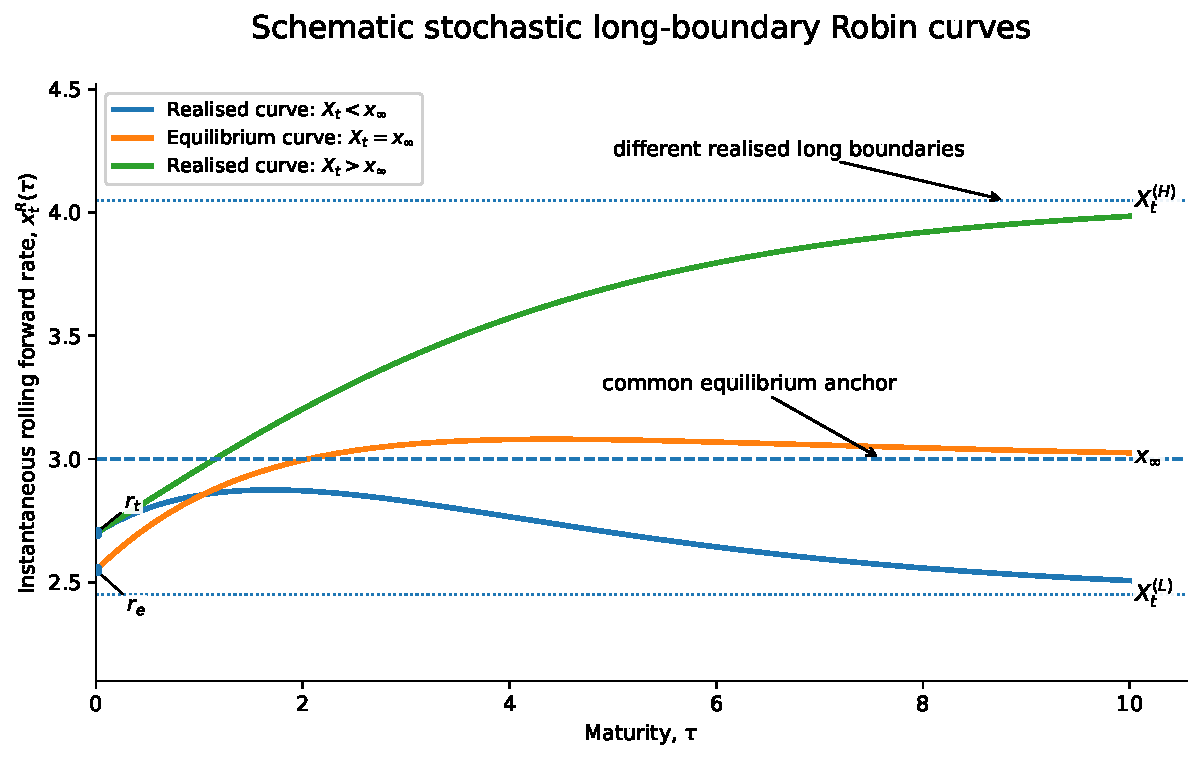
\includegraphics[width=0.78\textwidth]{UBFT_Paper_III_long_boundary_figure_v2.pdf}
 \caption{Schematic Robin curves drawn from different admissible initial boundary configurations with the same equilibrium anchor $x_\infty$. The upper and lower curves are not successive states of one trajectory: under the one-Brownian dynamics, the sign of $X_t-x_\infty$ is preserved at every finite time.}
 \label{fig:longboundary}
\end{figure}

\section{Robin closure and maturity loadings}

This section uses the Robin law to eliminate $D_t$ as an independent state.

\subsection{General continuous Robin law}

Impose the continuous mixed boundary condition
\begin{equation}
 \alpha_R x_t^R(0)
 +\beta_R\left.\frac{\partial x_t^R(\tau)}{\partial\tau}\right|_{\tau=0}
 =\gamma_R,
 \qquad \beta_R\neq0.
 \label{eq:generalrobin}
\end{equation}
The coefficient $\alpha_R$ multiplies the boundary level and $\beta_R$ multiplies the boundary slope. Thus the limiting cases $\beta_R=0$ and $\alpha_R=0$ are respectively Dirichlet and Neumann, while a genuine Robin condition combines both components. These coefficients are not probability weights: multiplying $(\alpha_R,\beta_R,\gamma_R)$ by the same non-zero constant leaves the boundary law unchanged, and the level and slope terms have different units. Only the ratios $\alpha_R/\beta_R$ and $\gamma_R/\beta_R$ are material. Dividing by $\beta_R$ gives
\begin{equation}
 \left.\frac{\partial x_t^R(\tau)}{\partial\tau}\right|_{\tau=0}
 +\frac{\alpha_R}{\beta_R}x_t^R(0)
 =\frac{\gamma_R}{\beta_R}.
 \label{eq:normalizedrobin}
\end{equation}
Section 7 shows that $\alpha_R/\beta_R=a^2(1-\kappa_R)$, so the Paper II parameter $\kappa_R$ is the dimensionless parameter controlling the relative level and slope contribution of the Robin operator.

From \eqref{eq:relaxedansatz},
\begin{equation}
 \left.\frac{\partial x_t^R(\tau)}{\partial\tau}\right|_{\tau=0}
 =D_t-a^2(r_t-X_t).
\end{equation}
Hence
\begin{equation}
 {
 D_t
 =a^2(r_t-X_t)+\frac{\gamma_R-\alpha_Rr_t}{\beta_R}.
 }
 \label{eq:Dtgeneral}
\end{equation}
The repeated-root coefficient is therefore not an independent stochastic primitive: the Robin law makes it affine in the short and long boundary states.

Substitution into \eqref{eq:relaxedansatz} shows that the curve is an affine maturity projection of the two boundary states,
\begin{equation}
 x_t^R(\tau)=L_r(\tau)r_t+L_X(\tau)X_t+L_0(\tau),
 \label{eq:loadingrepresentation}
\end{equation}
where
\begin{align}
 L_r(\tau)
 &=\left[1+\left(a^2-\frac{\alpha_R}{\beta_R}\right)\tau\right]e^{-a^2\tau},
 \label{eq:Lr}\\
 L_X(\tau)
 &=1-e^{-a^2\tau}-a^2\tau e^{-a^2\tau},
 \label{eq:LX}\\
 L_0(\tau)
 &=\frac{\gamma_R}{\beta_R}\tau e^{-a^2\tau}.
 \label{eq:L0}
\end{align}
At $\tau=0$ the loadings reduce to $(1,0,0)$, while as $\tau\to\infty$ they converge to $(0,1,0)$. Thus the field connects the realised short and long boundaries while preserving the repeated-root Robin geometry.

\subsection{Equilibrium curve}

Let
\begin{equation}
 r_e:=x_e^R(0),
 \qquad X_e=x_\infty.
\end{equation}
The equilibrium repeated-root coefficient is
\begin{equation}
 {
 D_e
 =\left(a^2-\frac{\alpha_R}{\beta_R}\right)r_e
 -a^2x_\infty
 +\frac{\gamma_R}{\beta_R}.
 }
 \label{eq:De}
\end{equation}
The equilibrium field is
\begin{equation}
 x_e^R(\tau)=L_r(\tau)r_e+L_X(\tau)x_\infty+L_0(\tau).
 \label{eq:eqcurve}
\end{equation}
Therefore
\begin{equation}
 {
 x_t^R(\tau)-x_e^R(\tau)
 =L_r(\tau)(r_t-r_e)+L_X(\tau)(X_t-x_\infty).
 }
 \label{eq:displacement}
\end{equation}
The deterministic Robin term $L_0$ cancels from the realised displacement.

\section{The Axiom-2 common kernel}

This section constructs the state-and-maturity kernel that the projected field diffusion must reproduce.

Differentiate \eqref{eq:eqcurve}. A direct calculation gives
\begin{equation}
 \frac{\partial x_e^R(\tau)}{\partial\tau}
 =e^{-a^2\tau}
 \left[
 \frac{\gamma_R-\alpha_Rr_e}{\beta_R}
 -a^2D_e\tau
 \right].
 \label{eq:eqderivative}
\end{equation}
Combining \eqref{eq:Qdefinition}, \eqref{eq:displacement} and \eqref{eq:eqderivative}, the exact rolling kernel is
\begin{align}
 Q_t(\tau)
 ={}&a(X_t-x_\infty)
 \nonumber\\
 &+e^{-a^2\tau}
 \left[
 a(r_t-r_e)-a(X_t-x_\infty)
 +\frac{\gamma_R-\alpha_Rr_e}{a\beta_R}
 \right]
 \nonumber\\
 &+a\tau e^{-a^2\tau}
 \left[
 \left(a^2-\frac{\alpha_R}{\beta_R}\right)(r_t-r_e)
 -a^2(X_t-x_\infty)-D_e
 \right].
 \label{eq:Qexpanded}
\end{align}
The maturity basis is therefore
\begin{equation}
 1,\qquad e^{-a^2\tau},\qquad \tau e^{-a^2\tau}.
\end{equation}
At the boundaries,
\begin{align}
 Q_t(0)
 &=a(r_t-r_e)+\frac{\gamma_R-\alpha_Rr_e}{a\beta_R},
 \label{eq:Qshort}\\
 \lim_{\tau\to\infty}Q_t(\tau)
 &=a(X_t-x_\infty).
 \label{eq:Qlong}
\end{align}
These expressions show why the short-boundary diffusion cannot in general be assumed to be simply $ar_t$: the rolling-equilibrium transport term is part of the common kernel.

\section{One Brownian field with two boundary states}

This section asks whether the two boundary states can share one Brownian innovation while preserving the Axiom-2 kernel at every maturity.

\subsection{Common-Brownian restriction}

Begin with the general state representation
\begin{equation}
 dr_t=\mu_r(t)dt+\sigma_r(t)dW_t^r,
 \qquad
 dX_t=\mu_X(t)dt+\sigma_X(t)dW_t^X,
\end{equation}
with
\begin{equation}
 dW_t^r\,dW_t^X=\rho\,dt.
\end{equation}
The cross-sectional representation \eqref{eq:loadingrepresentation} is independent of the correlation specification.

Under the one-field restriction
\begin{equation}
 \rho=1,
\end{equation}
the Brownian increments may be represented, with common orientation, as
\begin{equation}
 dW_t^r=dW_t^X=dW_t.
\end{equation}
Thus
\begin{equation}
 dx_t^R(\tau)\big|_{\mathrm{diffusion}}
 =G_t(\tau)dW_t,
\end{equation}
where
\begin{equation}
 {
 G_t(\tau)=L_r(\tau)\sigma_r+L_X(\tau)\sigma_X.
 }
 \label{eq:Gdefinition}
\end{equation}
Expansion in the same maturity basis gives
\begin{align}
 G_t(\tau)
 ={}&\sigma_X
 +(\sigma_r-\sigma_X)e^{-a^2\tau}
 \nonumber\\
 &+\left[
 \left(a^2-\frac{\alpha_R}{\beta_R}\right)\sigma_r
 -a^2\sigma_X
 \right]\tau e^{-a^2\tau}.
 \label{eq:Gexpanded}
\end{align}

\subsection{Coefficient matching}

Axiom 2 requires the projected diffusion loading to equal the common kernel, under the normalization used here:
\begin{equation}
 \boxed{G_t(\tau)=Q_t(\tau).}
 \label{eq:GequalsQ}
\end{equation}
The three maturity functions $1$, $e^{-a^2\tau}$ and $\tau e^{-a^2\tau}$ are linearly independent. Matching their coefficients gives
\begin{align}
 \sigma_X&=a(X_t-x_\infty),
 \label{eq:sigmaX}\\
 \sigma_r&=a(r_t-r_e)+\frac{\gamma_R-\alpha_Rr_e}{a\beta_R},
 \label{eq:sigmar}
\end{align}
and the remaining deterministic compatibility condition
\begin{equation}
 \left(a^2-\frac{\alpha_R}{\beta_R}\right)
 \frac{\gamma_R-\alpha_Rr_e}{\beta_R}
 =-a^2D_e.
 \label{eq:compatibilitygeneral}
\end{equation}
The residual calculation is given in Appendix B.

\paragraph{Theorem 1 (one-Brownian Robin closure).}
For the stochastic-long-boundary representation \eqref{eq:relaxedansatz}, subject to the Robin law \eqref{eq:generalrobin}, suppose the short and long boundary coordinates share one Brownian increment. If the equilibrium coefficients satisfy \eqref{eq:compatibilitygeneral}, then
\begin{equation}
 G_t(\tau)=Q_t(\tau)\qquad\text{for every }\tau\geq0.
 \label{eq:identityalltau}
\end{equation}
The enlarged maturity representation therefore contains two economically distinct boundary coordinates but one instantaneous innovation direction. Section 7 shows that \eqref{eq:compatibilitygeneral} is exactly the Paper II Robin identification, rather than an additional equilibrium assumption. Section 8 further shows that the shifted boundary coordinates are pathwise proportional under this strict closure.

\section{The compatibility condition is exactly Paper II}

This section verifies that the coefficient relation required by the one-Brownian closure is already contained in Paper II.

The preceding theorem would be less useful if \eqref{eq:compatibilitygeneral} were a new restriction. It is not. It is the Paper II Robin identification in general boundary notation.

Paper II writes the fixed-long-boundary Robin affine line as
\begin{equation}
 B_{R,t}=\eta_R+\kappa_Ra^2A_{R,t},
 \label{eq:paper2line}
\end{equation}
where
\begin{equation}
 A_{R,t}=r_t-x_\infty.
\end{equation}
Comparing the slope of \eqref{eq:Dtgeneral} in the limit $X_t=x_\infty$ with \eqref{eq:paper2line} gives
\begin{equation}
 {
 a^2-\frac{\alpha_R}{\beta_R}=\kappa_Ra^2,
 }
 \label{eq:kappamap}
\end{equation}
or equivalently
\begin{equation}
 \frac{\alpha_R}{\beta_R}=a^2(1-\kappa_R).
\end{equation}
The intercept is
\begin{equation}
 {
 \eta_R=\frac{\gamma_R-\alpha_Rx_\infty}{\beta_R}.
 }
 \label{eq:etamap}
\end{equation}
Also define
\begin{equation}
 A_R^e=r_e-x_\infty,
 \qquad
 D_e=B_R^e=\eta_R+\kappa_Ra^2A_R^e.
\end{equation}
Now
\begin{equation}
 \frac{\gamma_R-\alpha_Rr_e}{\beta_R}
 =\eta_R-a^2(1-\kappa_R)A_R^e.
\end{equation}
Substituting these relations into \eqref{eq:compatibilitygeneral} gives
\begin{equation}
 \kappa_Ra^2
 \left[
 \eta_R-a^2(1-\kappa_R)A_R^e
 \right]
 =-a^2\left[
 \eta_R+\kappa_Ra^2A_R^e
 \right].
\end{equation}
After cancellation,
\begin{equation}
 (1+\kappa_R)\eta_R+\kappa_R^2a^2A_R^e=0.
\end{equation}
For $\kappa_R\neq-1$,
\begin{equation}
 {
 \eta_R
 =-\frac{\kappa_R^2}{1+\kappa_R}a^2A_R^e.
 }
 \label{eq:paper2identification}
\end{equation}
Consequently,
\begin{equation}
 {
 B_{R,t}
 =-\frac{\kappa_R^2}{1+\kappa_R}a^2A_R^e
 +\kappa_Ra^2A_{R,t},
 }
 \label{eq:paper2manifold}
\end{equation}
which is precisely the identified one-factor Robin manifold in Paper II \cite{OzaShortBoundary}.

Thus the stochastic-long-boundary coefficient matching does not add a new equilibrium restriction. It recovers the existing one.

\subsection{Policy-anchor translation}

Paper II \cite{OzaShortBoundary} also permits the fixed-long-boundary curve to be written
\begin{equation}
 x_t^R(\tau)
 =(1+w_R\tau)e^{-a^2\tau}r_t
 -w_R\tau e^{-a^2\tau}x_D
 +(1-e^{-a^2\tau})x_\infty.
 \label{eq:policyanchor}
\end{equation}
Matching its repeated-root coefficient to \eqref{eq:paper2line} gives
\begin{equation}
 w_R=\kappa_Ra^2
\end{equation}
and
\begin{equation}
 \eta_R=\kappa_Ra^2(x_\infty-x_D).
\end{equation}
Using \eqref{eq:paper2identification}, for $\kappa_R\neq0$,
\begin{equation}
 {
 x_D=x_\infty+\frac{\kappa_R}{1+\kappa_R}A_R^e
 =\frac{x_\infty+\kappa_Rr_e}{1+\kappa_R}.
 }
\end{equation}
This is the policy-anchor expression of the same intercept condition, not an independent restriction.

\section{Boundary dynamics and full field evolution}

Under the convention
\begin{equation}
 dx_t^R(\tau)=-aQ_t(\tau)dt+Q_t(\tau)dW_t,
 \label{eq:fieldsde}
\end{equation}
the boundary dynamics follow by taking $\tau=0$ and $\tau\to\infty$.

At the long boundary,
\begin{equation}
 {
 dX_t
 =-a^2(X_t-x_\infty)dt
 +a(X_t-x_\infty)dW_t.
 }
 \label{eq:longsde}
\end{equation}
At the short boundary,
\begin{align}
 dr_t
 ={}&-a\left[
 a(r_t-r_e)+\frac{\gamma_R-\alpha_Rr_e}{a\beta_R}
 \right]dt
 \nonumber\\
 &+\left[
 a(r_t-r_e)+\frac{\gamma_R-\alpha_Rr_e}{a\beta_R}
 \right]dW_t.
 \label{eq:shortsde}
\end{align}
The same kernel governs the drift and diffusion at each boundary and at every interior maturity.

\medskip
\noindent\textbf{Corollary 1 (preservation of the UBFT market signal-to-noise ratio).} Under the one-Brownian Robin closure, \eqref{eq:fieldsde} has drift loading $-aQ_t(\tau)$ and diffusion loading $Q_t(\tau)$. Therefore, under the market signal-to-noise ratio (MSNR) convention of Papers I and II,
\begin{equation}
 \operatorname{MSNR}_t^R(\tau)
 :=\frac{\left|-aQ_t(\tau)\right|}{\sqrt{2}\left|Q_t(\tau)\right|}
 =\frac{a}{\sqrt{2}},
 \label{eq:msnrpreserved}
\end{equation}
for every maturity and admissible state at which $Q_t(\tau)\neq0$, with the value at a degeneracy boundary understood by continuity. Introducing a stochastic realised long boundary therefore preserves the maturity-, time- and state-independent MSNR of the earlier UBFT construction.
\medskip

Equation \eqref{eq:fieldsde} is the fixed-remaining-maturity form. For a fixed calendar maturity $T$, with $\tau=T-t$, It\^o's formula gives
\begin{equation}
 d x_{t,T}^R
 =\left[-aQ_t(\tau)-\frac{\partial x_t^R(\tau)}{\partial\tau}\right]dt
 +Q_t(\tau)dW_t.
 \label{eq:fixedTfield}
\end{equation}
Thus the change of coordinates adds the deterministic roll term $-\partial_\tau x_t^R(\tau)dt$ and does not alter the common diffusion kernel. Appendix C derives \eqref{eq:fixedTfield} directly.

With $Y_t=X_t-x_\infty$, \eqref{eq:longsde} gives
\begin{equation}
 Y_t=Y_{t_0}\exp\left[-\frac32a^2(t-t_0)+a(W_t-W_{t_0})\right].
\end{equation}
Hence, if $X_{t_0}>x_\infty$, then $X_t>x_\infty$ at every finite time almost surely. The equilibrium boundary $x_\infty$ is inaccessible from that admissible interior. Moreover,
\begin{align}
 \E_{t_0}[X_t-x_\infty]
 &=(X_{t_0}-x_\infty)e^{-a^2(t-t_0)},\\
 \E_{t_0}[(X_t-x_\infty)^2]
 &=(X_{t_0}-x_\infty)^2e^{-a^2(t-t_0)}.
\end{align}


\subsection{Pathwise relation between the boundary coordinates}

Define
\begin{equation}
 U_t:=r_t-r_e+\frac{\gamma_R-\alpha_Rr_e}{a^2\beta_R},
 \qquad
 Y_t:=X_t-x_\infty.
 \label{eq:UYdefinition}
\end{equation}
Equations \eqref{eq:longsde} and \eqref{eq:shortsde} imply
\begin{equation}
 dU_t=-a^2U_tdt+aU_tdW_t,
 \qquad
 dY_t=-a^2Y_tdt+aY_tdW_t.
 \label{eq:UYdynamics}
\end{equation}
Thus both shifted boundaries carry the same multiplicative stochastic state.

\paragraph{Proposition 2 (pathwise boundary-state relation).}
Under the one-Brownian boundary dynamics,
\begin{equation}
 U_tY_{t_0}=Y_tU_{t_0}
 \label{eq:pathwiseboundaryrelation}
\end{equation}
at every finite time almost surely. Whenever $Y_{t_0}\neq0$,
\begin{equation}
 \frac{U_t}{Y_t}=\frac{U_{t_0}}{Y_{t_0}}.
 \label{eq:constantboundaryratio}
\end{equation}
Accordingly, the curve representation contains two economically distinct boundary coordinates, but conditional on the initial boundary configuration the strict one-Brownian closure has only one dynamically independent stochastic coordinate. If either shifted boundary begins at zero, it remains there; otherwise its sign is preserved at every finite time.

Both components $X_t>x_\infty$ and $X_t<x_\infty$ are invariant under \eqref{eq:longsde}; a single trajectory cannot cross the equilibrium anchor. The positivity result below concerns the upper component $X_t\geq x_\infty$. Empirical crossings would require a moving anchor, a regime transition, or a boundary diffusion outside the strict closure studied here.

\section{Positivity inherited from the Paper II Robin field}

Paper II identifies the admissible Robin state region in which the fixed-long-boundary curve remains positive. The stochastic-long-boundary extension does not require that classification to be repeated when $X_t\geq x_\infty$. It is enough to compare the enlarged curve with the Paper II curve while preserving the same Robin parameters and the same short-boundary state.

Let
\begin{equation}
 B_{R,t}^{\mathrm{II}}:=\eta_R+\kappa_Ra^2A_{R,t},
 \qquad A_{R,t}=r_t-x_\infty,
\end{equation}
be the repeated-root coefficient of the Paper II curve. Using \eqref{eq:kappamap} and \eqref{eq:etamap}, the coefficient \eqref{eq:Dtgeneral} in the enlarged field becomes
\begin{equation}
 D_t=B_{R,t}^{\mathrm{II}}-a^2(X_t-x_\infty).
 \label{eq:Dtpositivity}
\end{equation}
Thus the Robin law is preserved as $X_t$ changes: $D_t$ is not held fixed, but adjusts by the explicit amount $-a^2(X_t-x_\infty)$. No dependence on $X_t$ is absorbed into $\kappa_R$, $\eta_R$, $A_{R,t}$ or the Paper II policy anchor.

Substituting \eqref{eq:Dtpositivity} into \eqref{eq:relaxedansatz} gives
\begin{align}
 x_t^R(\tau;X_t)
 ={}&x_t^{R,\mathrm{II}}(\tau)
 \nonumber\\
 &+(X_t-x_\infty)
 \left[1-(1+a^2\tau)e^{-a^2\tau}\right],
 \label{eq:positivitycomparison}
\end{align}
where
\begin{equation}
 x_t^{R,\mathrm{II}}(\tau)
 =x_\infty+
 \left[r_t-x_\infty+B_{R,t}^{\mathrm{II}}\tau\right]e^{-a^2\tau}
\end{equation}
is exactly the corresponding Paper II Robin curve. Since $e^z\geq1+z$ for $z\geq0$,
\begin{equation}
 1-(1+a^2\tau)e^{-a^2\tau}\geq0
 \qquad(\tau\geq0).
\end{equation}
Therefore, whenever $X_t\geq x_\infty$,
\begin{equation}
 x_t^R(\tau;X_t)\geq x_t^{R,\mathrm{II}}(\tau)
 \qquad\text{for every }\tau\geq0.
\end{equation}
Accordingly, positivity of the admissible Paper II Robin curve implies positivity of the stochastic-long-boundary curve throughout the same admissible short-boundary state region. Together with the sign preservation of $X_t-x_\infty$, this positivity inheritance holds pathwise at every finite time when $X_{t_0}>x_\infty$.

\section{Covariance rank and boundary-state dimension}

Under \eqref{eq:fieldsde}, every maturity is driven by the same Brownian increment. Therefore
\begin{equation}
 {
 \frac{\Cov_t(dx_t^R(\tau_1),dx_t^R(\tau_2))}{dt}
 =Q_t(\tau_1)Q_t(\tau_2).
 }
 \label{eq:rankonekernel}
\end{equation}
The instantaneous maturity covariance kernel is rank one.

This establishes the central distinction between curve geometry and stochastic dimension. The maturity representation contains two boundary coordinates, but Proposition 2 shows that their shifted forms are pathwise proportional. Conditional on the initial boundary ratio, the strict closure therefore has one dynamically independent stochastic state, one Brownian direction and rank-one instantaneous covariance.

The earlier fixed-long-boundary theory is recovered by imposing
\begin{equation}
 X_t\equiv x_\infty.
\end{equation}
That restriction removes a state coordinate. It is stronger than merely requiring the state covariance to be rank one.

\section{Comparison to familiar families of term-structure constructions}

Classical one-state equilibrium models make the term structure a function of a single short-rate diffusion and a fixed long-run parameter as is the case for the Vasicek model \cite{Vasicek1977}. HJM instead permits a stochastic forward-rate field driven by one or more Brownian motions, with no-arbitrage determining the risk-neutral drift from the chosen volatility structure \cite{HJM1992}. When a long-run level is promoted to a stochastic state in related short-rate extensions, it is commonly counted as an additional state factor.

The present construction occupies a different position. Within the UBFT repeated-root Robin representation, a stochastic realised long boundary is introduced without increasing Brownian dimension, and the coefficient compatibility required for that closure reproduces the existing Paper II Robin manifold. This is the narrow novelty claim advanced here; no broader claim of uniqueness among one-Brownian term-structure models is made.

\section{Imperfect correlation as an extension}

The cross-sectional representation \eqref{eq:loadingrepresentation} also permits a broader covariance specification with
\begin{equation}
 dW_t^r\,dW_t^X=\rho\,dt,
 \qquad |\rho|<1.
\end{equation}
Then
\begin{equation}
 dx_t^R(\tau)\big|_{\mathrm{diffusion}}
 =L_r(\tau)\sigma_r dW_t^r+L_X(\tau)\sigma_XdW_t^X.
\end{equation}
Provided both amplitudes are non-zero and the two maturity loadings are non-collinear, this produces a rank-two maturity covariance kernel. It collapses continuously to the one-field model as $\rho\to1$ with common Brownian orientation.

This broader system is mathematically admissible as an extension of the boundary-state representation. It should not, however, be presented as the necessary consequence of allowing $X_t$ to be stochastic. The one-Brownian Axiom-2 closure studied in this paper is the $\rho=1$ common-field case established above.

A second empirical covariance direction may also arise from movement in the Robin law itself, for example through time variation in $\kappa_R$, $x_D$, or their effective affine combination. That possibility is distinct from an independent long-end Brownian shock and should be tested separately in empirical work.

\section{Implications for the empirical programme}

The strict one-Brownian closure yields two complementary empirical restrictions. First, conditional on a locally stable Robin law, the shifted boundary series defined in \eqref{eq:UYdefinition} satisfy
\begin{equation}
 \frac{U_t}{X_t-x_\infty}=\text{constant}
 \label{eq:empiricalratio}
\end{equation}
over each interval on which the parameters and initial boundary configuration remain stable. Equivalently, where both shifted series are non-zero, $\log|U_t|-\log|X_t-x_\infty|$ is constant. Second, fitted curve innovations obey the rank-one covariance kernel \eqref{eq:rankonekernel}.

The pathwise proportionality restriction is a within-configuration statement. It applies on intervals over which the Robin coefficients, the equilibrium anchor and the initial boundary configuration may reasonably be treated as stable. Such intervals need not coincide with broad monetary-policy regimes or with a small ex ante number of statistical branches. The present theory does not itself provide a unique statistical rule for identifying those intervals.

A direct empirical sequence is nevertheless available. One first estimates $r_t$, $X_t$ and the Robin parameters from the curve, and then examines the trajectory of the boundary-law coordinates, particularly $\kappa_R$ and $x_D$, for locally stable configurations. Only after those intervals have been identified independently should one construct $U_t$ and test the local constancy of \eqref{eq:empiricalratio}. One may then test the rank of fitted curve innovations. Apparent rejection over a broad sample or a coarsely defined branch may reflect movement in the Robin law, movement in $x_\infty$, changes in the equilibrium configuration, measurement error, or aggregation across locally distinct branches, rather than failure of the within-configuration proportionality result.

The empirical coordinates used in companion work remain useful, but their interpretation changes. A near-rank-two Robin triangle need not mean that the short and long boundaries are primitive independent factors. It may instead reflect one curve-field innovation together with one boundary-law innovation. The parameters $\kappa_R$ and $x_D$ are therefore natural candidate coordinates for identifying changes in the boundary law, but whether they supply a reproducible regime classification is an empirical question rather than a result established here.

\section{Conclusion}

The fixed realised long boundary in the earlier UBFT papers was embedded in a natural but stronger-than-necessary cross-sectional ansatz. Because the maturity modes decayed around the constant $x_\infty$, the realised infinite-maturity state was fixed there pathwise. The axioms identify $x_\infty$ as the equilibrium long anchor, but do not themselves require that pathwise equality.

The minimally relaxed Robin field is
\begin{equation}
 x_t^R(\tau)=X_t+[r_t-X_t+D_t\tau]e^{-a^2\tau},
\end{equation}
with $D_t$ determined by the mixed short-boundary law. The resulting curve is affine in the short and long boundary coordinates. Applying Axiom 2 consistently shows that the one-Brownian projection closes exactly at every maturity:
\begin{equation}
 G_t(\tau)=Q_t(\tau).
\end{equation}
The deterministic coefficient relation required by that identity is precisely the Paper II Robin identification. No new equilibrium restriction is introduced.

Paper III therefore does not append a second Brownian factor to the earlier theory. It removes an implicit boundary closure and then reapplies the original axiomatic machinery. The resulting maturity representation has two economically distinct boundary coordinates, while the strict Axiom-2 dynamics make their shifted forms pathwise proportional. Conditional on the initial boundary configuration, the model therefore has one dynamically independent stochastic coordinate, one Brownian innovation direction and rank-one instantaneous covariance. An imperfect-correlation model remains available as a broader extension, but it is not required by stochasticity of $X_t$ itself.


\section*{AI-assisted research and drafting disclosure}
The author used OpenAI's ChatGPT as a research and drafting assistant during the development of this paper. Its contributions included algebraic checking, identification of structural implications, editorial review, figure preparation and LaTeX drafting. All mathematical claims, interpretations and final wording were reviewed and revised by the author, who takes full responsibility for the content of the paper.

\begin{appendices}

\section{Finite rolling-interval Robin limit}

At a final tradable rolling interval $\Delta t>0$, write
\begin{equation}
 x_t^R(\tau)=X_t+[r_t-X_t+D_t\tau]e^{-a^2\tau}.
\end{equation}
Then
\begin{equation}
 \left.\frac{\partial x_t^R(\tau)}{\partial\tau}\right|_{\tau=\Delta t}
 =[D_t-a^2(r_t-X_t)-a^2D_t\Delta t]e^{-a^2\Delta t}.
\end{equation}
Imposing
\begin{equation}
 \alpha_Rx_t^R(\Delta t)
 +\beta_R\left.\frac{\partial x_t^R(\tau)}{\partial\tau}\right|_{\tau=\Delta t}
 =\gamma_R
\end{equation}
and taking $\Delta t\downarrow0$ yields \eqref{eq:generalrobin} and \eqref{eq:Dtgeneral}.

\section{Residual in the coefficient match}

With \eqref{eq:sigmaX} and \eqref{eq:sigmar}, the difference between the projected diffusion and the Axiom-2 kernel is
\begin{equation}
 \begin{aligned}
 G_t(\tau)-Q_t(\tau)
 ={}&\tau e^{-a^2\tau}
 \Bigg[
 \left(a^2-\frac{\alpha_R}{\beta_R}\right)
 \frac{\gamma_R-\alpha_Rr_e}{a\beta_R}
 +aD_e
 \Bigg].
 \end{aligned}
\end{equation}
Thus $G_t(\tau)=Q_t(\tau)$ for all $\tau$ if and only if \eqref{eq:compatibilitygeneral} holds.

\section{\texorpdfstring{Fixed-$\tau$ and fixed-$T$ forms}{Fixed-tau and fixed-T forms}}

Let $\widetilde x(t,\tau)$ denote the rolling field, so that the fixed-calendar-maturity process is
\begin{equation}
 x_{t,T}^R=\widetilde x(t,T-t).
\end{equation}
At fixed $\tau$, \eqref{eq:fieldsde} gives
\begin{equation}
 d\widetilde x(t,\tau)
 =-aQ_t(\tau)dt+Q_t(\tau)dW_t.
\end{equation}
For fixed $T$, $d\tau=d(T-t)=-dt$. Applying It\^o's formula to $\widetilde x(t,T-t)$ therefore yields
\begin{align}
 d x_{t,T}^R
 &=d\widetilde x(t,\tau)
 +\frac{\partial\widetilde x(t,\tau)}{\partial\tau}d\tau
 \nonumber\\
 &=\left[-aQ_t(\tau)-\frac{\partial x_t^R(\tau)}{\partial\tau}\right]dt
 +Q_t(\tau)dW_t.
\end{align}
The coordinate transformation changes only the deterministic drift through the roll term. The maturity diffusion remains $Q_t(\tau)$, so the one-Brownian coefficient matching is invariant to the choice of fixed-$\tau$ or fixed-$T$ coordinates.

\section{Infinite-maturity generator}

For \eqref{eq:longsde}, the generator acting on a smooth test function $\varphi$ is
\begin{equation}
 (\mathcal A\varphi)(X)
 =-a^2(X-x_\infty)\varphi'(X)
 +\frac12a^2(X-x_\infty)^2\varphi''(X).
\end{equation}
Applying it to $\varphi(X)=(X-x_\infty)^2$ gives
\begin{equation}
 (\mathcal A\varphi)(X)=-a^2(X-x_\infty)^2,
\end{equation}
which yields the stated second-moment decay.

\section{Normalization convention}

The paper uses
\begin{equation}
 dx_t^R(\tau)=-aQ_t(\tau)dt+Q_t(\tau)dW_t.
\end{equation}
Equivalently, one may factor $Q_t=a\mathcal K_t$ and write
\begin{equation}
 dx_t^R(\tau)=-a^2\mathcal K_t(\tau)dt+a\mathcal K_t(\tau)dW_t.
\end{equation}
The factor $\sqrt2$ used in the Paper II MSNR convention belongs to its separate second-moment noise-scale definition. It is not inserted into the Brownian coefficient.

\section{Risk-neutral compatibility}

The main text concerns physical-measure axiomatic consistency. It does not establish a complete arbitrage-free pricing model, prove the existence of an equivalent martingale measure, or derive the admissibility of the infinite-maturity boundary under that measure. Under an equivalent pricing measure, the maturity volatility would retain the boundary loading up to measure-consistent parameterisation, while the no-arbitrage drift would be determined by the corresponding HJM restriction. This appendix therefore records the intended pricing interface rather than a complete risk-neutral compatibility theorem.

\end{appendices}

\begin{thebibliography}{9}
\bibitem{OzaIRFR}
Oza, S. (2026).
\newblock An Axiomatically Consistent Single-Factor Term Structure Model with Admissible Humped Volatility.
\newblock April 30, 2026. Available at SSRN: \url{https://ssrn.com/abstract=6748347}; DOI: \url{https://doi.org/10.2139/ssrn.6748347}.

\bibitem{OzaShortBoundary}
Oza, S. (2026).
\newblock Unified Boundary Field Theory II: Monetary Policy as a Short-End Boundary Condition.
\newblock June 26, 2026. Available at SSRN: \url{https://ssrn.com/abstract=6454299}; DOI: \url{https://doi.org/10.2139/ssrn.6454299}.


\bibitem{Vasicek1977}
Vasicek, O. (1977).
\newblock An Equilibrium Characterization of the Term Structure.
\newblock \emph{Journal of Financial Economics}, 5(2), 177--188.

\bibitem{HJM1992}
Heath, D., Jarrow, R. and Morton, A. (1992).
\newblock Bond Pricing and the Term Structure of Interest Rates: A New Methodology for Contingent Claims Valuation.
\newblock \emph{Econometrica}, 60(1), 77--105.

\end{thebibliography}

\end{document}
